% !TEX program = LuaLaTeX
%%%%%%%%%%%%%%%%%%%%%%%%%%%%%%%%%%%%%%%%%%%%%%%%%%%%%%%%%%%%%%%%%%%%%%%%%%%%%%
\RequirePackage{luatex85}
\documentclass[%
  lualatex,
  ja=standard,
  textwidth-limit=60,
  a4paper, 12pt,
  %b5paper,
  oneside,
  everyparhook=compat]{bxjsarticle}

\usepackage{graphicx}

% Default preamble
\usepackage{pgfplots}
\pgfplotsset{compat=newest}
\usepgfplotslibrary{groupplots}
\usepgfplotslibrary{polar}
\usepgfplotslibrary{smithchart}
\usepgfplotslibrary{statistics}
\usepgfplotslibrary{dateplot}
\usepgfplotslibrary{ternary}

% Custom preamble
\usetikzlibrary{arrows.meta}
\usetikzlibrary{backgrounds}
\usepgfplotslibrary{patchplots}
\usepgfplotslibrary{fillbetween}

%%%%%%%%%%%%%%%%%%%%%%%%%%%%%%%%%%%%%%%%%%%%%%%%%%%%%%%%%%%%%%%%%%%%%%%%%%%%%%
\begin{document}

\begin{figure}[htbp]
\centering
\scalebox{0.7}{% Recommended preamble:
% \usetikzlibrary{arrows.meta}
% \usetikzlibrary{backgrounds}
% \usepgfplotslibrary{patchplots}
% \usepgfplotslibrary{fillbetween}
% \pgfplotsset{%
%     layers/standard/.define layer set={%
%         background,axis background,axis grid,axis ticks,axis lines,axis tick labels,pre main,main,axis descriptions,axis foreground%
%     }{
%         grid style={/pgfplots/on layer=axis grid},%
%         tick style={/pgfplots/on layer=axis ticks},%
%         axis line style={/pgfplots/on layer=axis lines},%
%         label style={/pgfplots/on layer=axis descriptions},%
%         legend style={/pgfplots/on layer=axis descriptions},%
%         title style={/pgfplots/on layer=axis descriptions},%
%         colorbar style={/pgfplots/on layer=axis descriptions},%
%         ticklabel style={/pgfplots/on layer=axis tick labels},%
%         axis background@ style={/pgfplots/on layer=axis background},%
%         3d box foreground style={/pgfplots/on layer=axis foreground},%
%     },
% }

\begin{tikzpicture}[/tikz/background rectangle/.style={fill={rgb,1:red,1.0;green,1.0;blue,1.0}, fill opacity={1.0}, draw opacity={1.0}}, show background rectangle]
\begin{axis}[point meta max={nan}, point meta min={nan}, legend cell align={left}, legend columns={1}, title={\textbf{こんな感じに日本語をpgfplotsx()でも使えます!}}, title style={at={{(0.5,1)}}, anchor={south}, font={{\fontsize{17 pt}{22.1 pt}\selectfont}}, color={rgb,1:red,0.0;green,0.0;blue,0.0}, draw opacity={1.0}, rotate={0.0}, align={center}}, legend style={color={rgb,1:red,0.0;green,0.0;blue,0.0}, draw opacity={1.0}, line width={1}, solid, fill={rgb,1:red,1.0;green,1.0;blue,1.0}, fill opacity={1.0}, text opacity={1.0}, font={{\fontsize{15 pt}{19.5 pt}\selectfont}}, text={rgb,1:red,0.0;green,0.0;blue,0.0}, cells={anchor={center}}, at={(0.02, 0.98)}, anchor={north west}}, axis background/.style={fill={rgb,1:red,1.0;green,1.0;blue,1.0}, opacity={1.0}}, anchor={north west}, xshift={1.0mm}, yshift={-1.0mm}, width={150.4mm}, height={99.6mm}, scaled x ticks={false}, xlabel={$\theta$}, x tick style={color={rgb,1:red,0.0;green,0.0;blue,0.0}, opacity={1.0}}, x tick label style={color={rgb,1:red,0.0;green,0.0;blue,0.0}, opacity={1.0}, rotate={0}}, xlabel style={at={(ticklabel cs:0.5)}, anchor=near ticklabel, at={{(ticklabel cs:0.5)}}, anchor={near ticklabel}, font={{\fontsize{14 pt}{18.2 pt}\selectfont}}, color={rgb,1:red,0.0;green,0.0;blue,0.0}, draw opacity={1.0}, rotate={0.0}}, xmajorgrids={true}, xmin={-5.300000000000001}, xmax={5.300000000000001}, xticklabels={{$-2\pi$,$-3\pi/2$,$-\pi$,$-\pi/2$,$0$,$\pi/2$,$\pi$,$3\pi/2$,$2\pi$}}, xtick={{-6.283185307179586,-4.71238898038469,-3.141592653589793,-1.5707963267948966,0.0,1.5707963267948966,3.141592653589793,4.71238898038469,6.283185307179586}}, xtick align={inside}, xticklabel style={font={{\fontsize{14 pt}{18.2 pt}\selectfont}}, color={rgb,1:red,0.0;green,0.0;blue,0.0}, draw opacity={1.0}, rotate={0.0}}, x grid style={color={rgb,1:red,0.0;green,0.0;blue,0.0}, draw opacity={0.1}, line width={0.5}, solid}, axis x line*={left}, x axis line style={color={rgb,1:red,0.0;green,0.0;blue,0.0}, draw opacity={1.0}, line width={1}, solid}, scaled y ticks={false}, ylabel={$y$}, y tick style={color={rgb,1:red,0.0;green,0.0;blue,0.0}, opacity={1.0}}, y tick label style={color={rgb,1:red,0.0;green,0.0;blue,0.0}, opacity={1.0}, rotate={0}}, ylabel style={at={(ticklabel cs:0.5)}, anchor=near ticklabel, at={{(ticklabel cs:0.5)}}, anchor={near ticklabel}, font={{\fontsize{14 pt}{18.2 pt}\selectfont}}, color={rgb,1:red,0.0;green,0.0;blue,0.0}, draw opacity={1.0}, rotate={0.0}}, ymajorgrids={true}, ymin={-1.2}, ymax={1.4}, yticklabels={{$-1.0$,$-0.8$,$-0.6$,$-0.4$,$-0.2$,$0.0$,$0.2$,$0.4$,$0.6$,$0.8$,$1.0$}}, ytick={{-1.0,-0.8,-0.6,-0.4,-0.2,0.0,0.2,0.4,0.6,0.8,1.0}}, ytick align={inside}, yticklabel style={font={{\fontsize{14 pt}{18.2 pt}\selectfont}}, color={rgb,1:red,0.0;green,0.0;blue,0.0}, draw opacity={1.0}, rotate={0.0}}, y grid style={color={rgb,1:red,0.0;green,0.0;blue,0.0}, draw opacity={0.1}, line width={0.5}, solid}, axis y line*={left}, y axis line style={color={rgb,1:red,0.0;green,0.0;blue,0.0}, draw opacity={1.0}, line width={1}, solid}, colorbar={false}]
    \addplot[color={rgb,1:red,0.0;green,0.6056;blue,0.9787}, name path={5}, draw opacity={1.0}, line width={1}, solid]
        table[row sep={\\}]
        {
            \\
            -5.0  0.9589242746631385  \\
            -4.974190733787667  0.9659252140230418  \\
            -4.948381467575334  0.9722827687117676  \\
            -4.9225722013630016  0.9779927040813603  \\
            -4.896762935150669  0.9830512168509479  \\
            -4.82118167807464  0.99408790913608  \\
            -4.745600420998612  0.9994485507963324  \\
            -4.707809792460598  0.9999895155372986  \\
            -4.670019163922583  0.9991025335996101  \\
            -4.632228535384568  0.996788871559458  \\
            -4.594437906846554  0.993051833237507  \\
            -4.5566472783085405  0.9878967549811657  \\
            -4.518856649770526  0.9813309980444871  \\
            -4.481066021232511  0.9733639380765804  \\
            -4.443275392694497  0.9640069517335438  \\
            -4.405484764156483  0.9532734004330353  \\
            -4.367694135618469  0.9411786112746806  \\
            -4.329903507080454  0.9277398551535638  \\
            -4.29211287854244  0.9129763220980507  \\
            -4.221792100135206  0.8820517941566471  \\
            -4.15147132172797  0.8467673067333348  \\
            -4.081150543320735  0.8072972701479215  \\
            -4.010829764913501  0.7638367837827817  \\
            -3.96370173790384  0.7325830645529303  \\
            -3.9165737108941796  0.6997025421608782  \\
            -3.8694456838845195  0.6652682324056393  \\
            -3.822317656874859  0.6293566014883968  \\
            -3.7751896298651983  0.59204739620861  \\
            -3.7280616028555382  0.5534234668750911  \\
            -3.6809335758458777  0.5135705833253043  \\
            -3.633805548836217  0.4725772444614477  \\
            -3.555920958090951  0.40257515996388127  \\
            -3.4780363673456853  0.33013228492720376  \\
            -3.4001517766004197  0.2556878364258897  \\
            -3.3222671858551536  0.17969316696168675  \\
            -3.1774172901869173  0.03581697417168226  \\
            -3.0325673945186806  -0.10880939914913097  \\
            -2.941649212961252  -0.19861389852769232  \\
            -2.8507310314038232  -0.2867777630409597  \\
            -2.7598128498463947  -0.37257272185264245  \\
            -2.6688946682889663  -0.455290072290187  \\
            -2.5873405722830283  -0.5263074964545077  \\
            -2.50578647627709  -0.5938263520628001  \\
            -2.4242323802711514  -0.6573978152872416  \\
            -2.3426782842652134  -0.7165993021369216  \\
            -2.2960034482411404  -0.748362056340159  \\
            -2.2493286122170675  -0.7784947695893576  \\
            -2.2026537761929945  -0.8069318084705348  \\
            -2.1559789401689216  -0.8336112329940892  \\
            -2.1093041041448486  -0.8584749315090688  \\
            -2.0626292681207756  -0.8814687472787648  \\
            -2.0159544320967027  -0.9025425964419272  \\
            -1.9692795960726297  -0.9216505771026704  \\
            -1.8995007181568861  -0.9464613823435548  \\
            -1.8297218402411428  -0.9666656498187214  \\
            -1.7599429623253995  -0.9821650430055298  \\
            -1.690164084409656  -0.9928841245523959  \\
            -1.645539826164151  -0.9972080048253645  \\
            -1.600915567918646  -0.9995464499458205  \\
            -1.556291309673141  -0.999894804083564  \\
            -1.511667051427636  -0.9982523736675974  \\
            -1.467042793182131  -0.9946224287670216  \\
            -1.422418534936626  -0.9890121965803468  \\
            -1.3777942766911213  -0.9814328470461853  \\
            -1.3331700184456163  -0.9718994706039692  \\
            -1.2924412899312923  -0.9615087326987289  \\
            -1.2517125614169682  -0.9495232363810592  \\
            -1.210983832902644  -0.9359628607955058  \\
            -1.17025510438832  -0.9208500971814154  \\
            -1.0887976473596719  -0.8860702032046404  \\
            -1.0073401903310237  -0.8454142025055484  \\
            -0.9609858683859815  -0.8197565853313542  \\
            -0.9146315464409394  -0.7923378535737733  \\
            -0.8682772244958972  -0.7632169119482056  \\
            -0.8219229025508551  -0.732456322092943  \\
            -0.775568580605813  -0.7001221681655964  \\
            -0.7292142586607708  -0.6662839148719598  \\
            -0.6828599367157286  -0.6310142582323133  \\
            -0.6365056147706865  -0.5943889694057675  \\
            -0.5630133285022302  -0.5337368404088737  \\
            -0.48952104223377385  -0.4702032340313718  \\
            -0.4160287559653175  -0.404131148237474  \\
            -0.34253646969686125  -0.3358772854435974  \\
            -0.15992707331630546  -0.15924621097882932  \\
            0.02268232306425034  0.022680378151277828  \\
            0.16253160521297816  0.16181696314467953  \\
            0.302380887361706  0.2977939154893836  \\
            0.40096461053763316  0.3903066261397785  \\
            0.49954833371356033  0.479029115258919  \\
            0.5488401953015238  0.5216981156605566  \\
            0.5981320568894875  0.563099809237636  \\
            0.6474239184774511  0.6031336231737269  \\
            0.6967157800654147  0.6417023074997542  \\
            0.7703855963663375  0.6964120106137743  \\
            0.8440554126672604  0.7473438264196488  \\
            0.9177252289681832  0.7942214606295402  \\
            0.991395045269106  0.8367906120300602  \\
            1.03328460922588  0.8589853403273437  \\
            1.075174173182654  0.8796729968905124  \\
            1.117063737139428  0.8988172856607305  \\
            1.1589533010962023  0.9163846183855323  \\
            1.2008428650529765  0.9323441735487051  \\
            1.2427324290097506  0.9466679504459921  \\
            1.2846219929665246  0.9593308183117394  \\
            1.3265115569232986  0.9703105604102974  \\
            1.3679966116850608  0.9795065199638723  \\
            1.409481666446823  0.9870169809789519  \\
            1.450966721208585  0.9928290197324098  \\
            1.4924517759703473  0.9969326350832379  \\
            1.5339368307321095  0.9993207656821391  \\
            1.5754218854938715  0.9999893021224353  \\
            1.6169069402556338  0.9989370940113829  \\
            1.658391995017396  0.9961659519497252  \\
            1.70403315611983  0.9911370965289318  \\
            1.7496743172222642  0.9840439463580991  \\
            1.7953154783246983  0.9749012747241017  \\
            1.8409566394271324  0.9637281235628345  \\
            1.8865978005295665  0.9505477637995456  \\
            1.9322389616320006  0.9353876468812224  \\
            1.9778801227344347  0.9182793476019822  \\
            2.023521283836869  0.8992584983405417  \\
            2.093245213615395  0.8665997754981649  \\
            2.162969143393921  0.8297298480962021  \\
            2.232693073172447  0.7888278839705755  \\
            2.302417002950973  0.7440926444672856  \\
            2.390402610490068  0.6825090184381307  \\
            2.4783882180291634  0.6156451789762168  \\
            2.5663738255682587  0.5440184164524472  \\
            2.6543594331073534  0.46818286946925186  \\
            2.7357369398246343  0.3948051045883107  \\
            2.8171144465419147  0.3188142649405604  \\
            2.898491953259195  0.24071330690443776  \\
            2.979869459976476  0.1610191529825544  \\
            3.147723079235892  -0.006130387247107083  \\
            3.3155766984953083  -0.17310760996769  \\
            3.4006462095786185  -0.2561658028806896  \\
            3.4857157206619283  -0.33737128726303256  \\
            3.570785231745238  -0.4161367478214236  \\
            3.655854742828548  -0.4918925166335389  \\
            3.7446832705972923  -0.567190568916659  \\
            3.833511798366036  -0.6380161418542699  \\
            3.877926062250408  -0.6715757227513456  \\
            3.92234032613478  -0.7038107531135251  \\
            3.9667545900191516  -0.7346576557070549  \\
            4.0111688539035235  -0.7640555911061697  \\
            4.081143324377254  -0.8072930099035063  \\
            4.151117794850984  -0.8465791904397305  \\
            4.221092265324714  -0.8817218492963513  \\
            4.291066735798444  -0.9125489832272522  \\
            4.330905329400883  -0.9281132971615369  \\
            4.370743923003321  -0.9422047847257197  \\
            4.410582516605759  -0.9548010840868847  \\
            4.450421110208197  -0.9658822061317183  \\
            4.490259703810635  -0.9754305661873062  \\
            4.530098297413073  -0.983431011926315  \\
            4.5699368910155105  -0.9898708474122756  \\
            4.609775484617948  -0.9947398532468108  \\
            4.649614078220386  -0.9980303027868359  \\
            4.689452671822824  -0.9997369744059967  \\
            4.729291265425262  -0.9998571597808878  \\
            4.769129859027701  -0.9983906681889001  \\
            4.80896845263014  -0.9953398268108796  \\
            4.848807046232578  -0.9907094770381162  \\
            4.8886456398350155  -0.9845069667895209  \\
            4.9284842334374535  -0.9767421388511879  \\
            4.9463631750780905  -0.9727526811839345  \\
            4.964242116718727  -0.9684522850294619  \\
            4.982121058359363  -0.9638423250009686  \\
            5.0  -0.9589242746631385  \\
        }
        ;
    \addlegendentry {正弦関数 $y = \sin\theta$}
    \node[right, , color={rgb,1:red,1.0;green,0.0;blue,0.0}, draw opacity={1.0}, rotate={45.0}, font={{\fontsize{14 pt}{18.2 pt}\selectfont}}]  at (axis cs:0,-0.3) {正弦関数 $y = \sin\theta$};
\end{axis}
\end{tikzpicture}
}
\caption{pgfplotsx-ja-fig.tex}
\label{fig:pgfplotsx-ja-fig.tex}
\end{figure}

\noindent
図\ref{fig:pgfplotsx-ja-fig.tex}はPlots.jl pgfplotsx()で作ったtexファイルを読み込んで作った図である.

\begin{figure}[htbp]
\centering
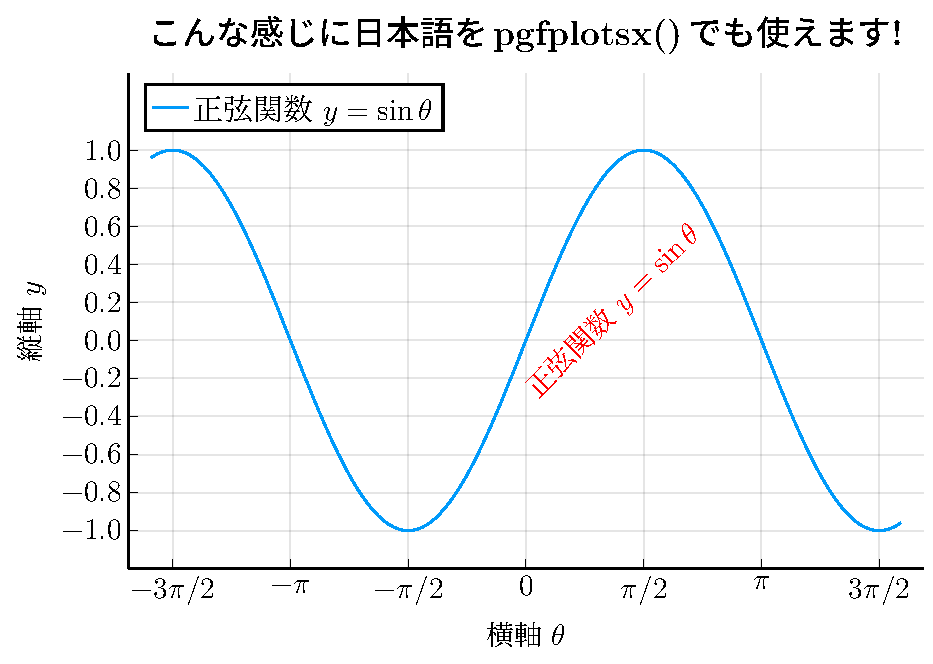
\includegraphics[width=0.7\columnwidth]{pgfplotsx-ja-fig.pdf}
\caption{pgfplotsx-ja-fig.pdf}
\label{fig:pgfplotsx-ja-fig.pdf}
\end{figure}

\noindent
図\ref{fig:pgfplotsx-ja-fig.pdf}はPlots.jl pgfplotsx()で作ったpdfファイルを読み込んだ結果である.

%%%%%%%%%%%%%%%%%%%%%%%%%%%%%%%%%%%%%%%%%%%%%%%%%%%%%%%%%%%%%%%%%%%%%%%%%%%%%%
\end{document}
